\documentclass{standalone}
\usepackage{tikz}
\usetikzlibrary{patterns}
\usetikzlibrary{positioning}
\usetikzlibrary{patterns, positioning}
\usetikzlibrary{shapes.misc}
\usepackage[outline]{contour}
\contourlength{1.5pt} 
\usepackage[sfdefault]{ClearSans}

\begin{document}
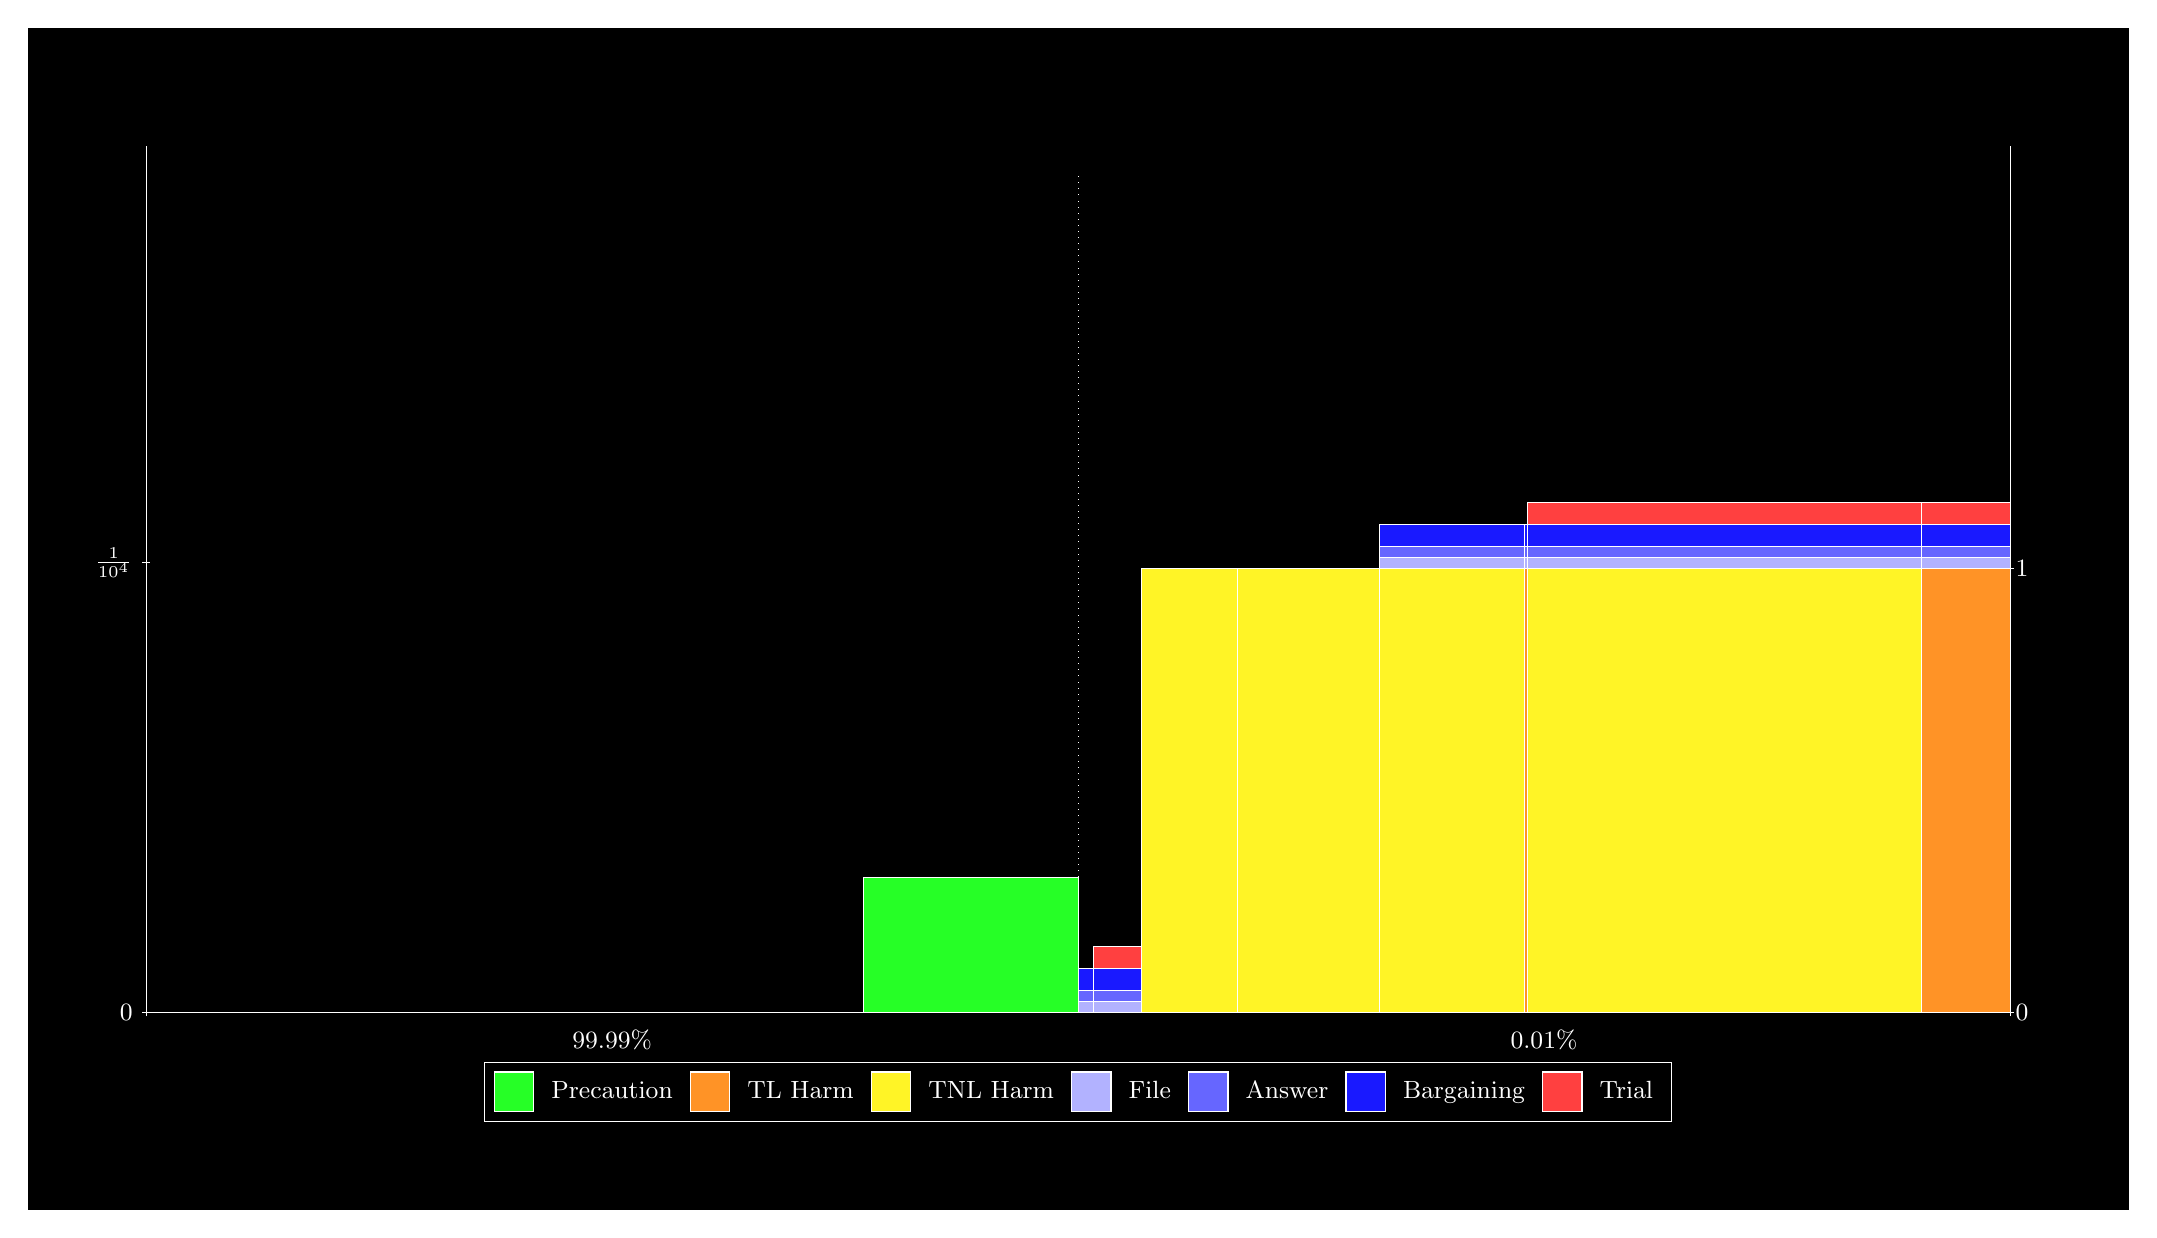
\begin{tikzpicture}
\draw[fill=black] (0,0) rectangle (26.667,15);
\draw[fill=green!85,draw=white,very thin] (10.611,2.5) rectangle (13.333,4.2141);
\draw[fill=blue!30,draw=white,very thin] (13.333,2.5) rectangle (13.522,2.6409);
\draw[fill=blue!60,draw=white,very thin] (13.333,2.6409) rectangle (13.522,2.7818);
\draw[fill=blue!90,draw=white,very thin] (13.333,2.7818) rectangle (13.522,3.0635);
\draw[fill=blue!30,draw=white,very thin] (13.522,2.5) rectangle (14.135,2.6409);
\draw[fill=blue!60,draw=white,very thin] (13.522,2.6409) rectangle (14.135,2.7818);
\draw[fill=blue!90,draw=white,very thin] (13.522,2.7818) rectangle (14.135,3.0635);
\draw[fill=red!75,draw=white,very thin] (13.522,3.0635) rectangle (14.135,3.3453);
\draw[fill=yellow!85,draw=white,very thin] (14.135,2.5) rectangle (15.36,8.1355);
\draw[fill=green!85,draw=white,very thin] (15.36,2.5) rectangle (17.153,2.5002);
\draw[fill=yellow!85,draw=white,very thin] (15.36,2.5002) rectangle (17.153,8.1356);
\draw[fill=yellow!85,draw=white,very thin] (17.153,2.5) rectangle (19.005,8.1355);
\draw[fill=blue!30,draw=white,very thin] (17.153,8.1355) rectangle (19.005,8.2764);
\draw[fill=blue!60,draw=white,very thin] (17.153,8.2764) rectangle (19.005,8.4173);
\draw[fill=blue!90,draw=white,very thin] (17.153,8.4173) rectangle (19.005,8.699);
\draw[fill=orange!85,draw=white,very thin] (19.005,2.5) rectangle (19.037,8.1355);
\draw[fill=blue!30,draw=white,very thin] (19.005,8.1355) rectangle (19.037,8.2764);
\draw[fill=blue!60,draw=white,very thin] (19.005,8.2764) rectangle (19.037,8.4173);
\draw[fill=blue!90,draw=white,very thin] (19.005,8.4173) rectangle (19.037,8.699);
\draw[fill=yellow!85,draw=white,very thin] (19.037,2.5) rectangle (24.046,8.1355);
\draw[fill=blue!30,draw=white,very thin] (19.037,8.1355) rectangle (24.046,8.2764);
\draw[fill=blue!60,draw=white,very thin] (19.037,8.2764) rectangle (24.046,8.4173);
\draw[fill=blue!90,draw=white,very thin] (19.037,8.4173) rectangle (24.046,8.699);
\draw[fill=red!75,draw=white,very thin] (19.037,8.699) rectangle (24.046,8.9808);
\draw[fill=orange!85,draw=white,very thin] (24.046,2.5) rectangle (25.167,8.1355);
\draw[fill=blue!30,draw=white,very thin] (24.046,8.1355) rectangle (25.167,8.2764);
\draw[fill=blue!60,draw=white,very thin] (24.046,8.2764) rectangle (25.167,8.4173);
\draw[fill=blue!90,draw=white,very thin] (24.046,8.4173) rectangle (25.167,8.699);
\draw[fill=red!75,draw=white,very thin] (24.046,8.699) rectangle (25.167,8.9808);
\draw[white,very thin] (1.5,2.5) -- (1.5,13.5);
\draw[white,very thin] (1.45,2.5) -- (1.55,2.5);
\node[font=\small,text=white, anchor=east] at (1.45, 2.5) {0};
\draw[white,very thin] (1.45,8.2138) -- (1.55,8.2138);
\node[font=\small,text=white, anchor=east] at (1.45, 8.2138) {$\frac{1}{10^{4}}$};

\draw[white,dotted,very thin] (13.333,2.83) -- (13.333,13.17);
\draw[white,very thin] (25.167,2.5) -- (25.167,13.5);
\draw[white,very thin] (25.117,2.5) -- (25.217,2.5);
\node[font=\small,text=white, anchor=west] at (25.117, 2.5) {0};
\draw[white,very thin] (25.117,8.1355) -- (25.217,8.1355);
\node[font=\small,text=white, anchor=west] at (25.117, 8.1355) {1};

\draw[white,very thin] (1.5,2.5) -- (25.167,2.5);
\draw[white,very thin] (1.5,2.45) -- (1.5,2.55);
\node[font=\small,text=white, anchor=north] at (1.5, 2.45) {};
\draw[white,very thin] (25.167,2.45) -- (25.167,2.55);
\node[font=\small,text=white, anchor=north] at (25.167, 2.45) {};

\node[font=\small,text=white,anchor=south] at (7.4167, 1.9) {99.99\%};
\node[font=\small,text=white,anchor=south] at (19.25, 1.9) {0.01\%};
\draw (13.3333,2.5) node (B) {};
\begin{scope}[align=center]
\matrix[scale=0.5,draw=white,below=0.5cm of B,nodes={draw},column sep=0.1cm]{
\node[rectangle,draw,minimum width=0.5cm,minimum height=0.5cm,fill=green!85]{}; & \node[draw=none,font=\small,text=white]{Precaution}; &
\node[rectangle,draw,minimum width=0.5cm,minimum height=0.5cm,fill=orange!85]{}; & \node[draw=none,font=\small,text=white]{TL Harm}; &
\node[rectangle,draw,minimum width=0.5cm,minimum height=0.5cm,fill=yellow!85]{}; & \node[draw=none,font=\small,text=white]{TNL Harm}; &
\node[rectangle,draw,minimum width=0.5cm,minimum height=0.5cm,fill=blue!30]{}; & \node[draw=none,font=\small,text=white]{File}; &
\node[rectangle,draw,minimum width=0.5cm,minimum height=0.5cm,fill=blue!60]{}; & \node[draw=none,font=\small,text=white]{Answer}; &
\node[rectangle,draw,minimum width=0.5cm,minimum height=0.5cm,fill=blue!90]{}; & \node[draw=none,font=\small,text=white]{Bargaining}; &
\node[rectangle,draw,minimum width=0.5cm,minimum height=0.5cm,fill=red!75]{}; & \node[draw=none,font=\small,text=white]{Trial}; \\\\
};\end{scope}

\end{tikzpicture}
\end{document}